\chapter{Preliminaries}
\label{chapter:preliminaries}

En este capítulo se explican los conceptos básicos de los temas que toman un
papel importante en el desarrollo del proyecto separados cada uno en secciones,
principalmente algoritmos genéticos siendo que este tema es la parte primordial
del proyecto, además de esto se explica de manera detallada los conceptos que se
tomaran en cuenta en el desarrollo de los métodos que componen el sistema,
siendo estos open-ended evolution, generación procedural de contenido, los
conceptos básicos de jugabilidad y la regla de los tercios.

\section{Algoritmos genéticos}
\label{section:financial-market}

A financial market is constructed by the interaction of a number of traders,
where a trader is an entity that is able to buy or sell a number of units of an
asset \cite{Huang2009}. The entities defined as traders can either be individual
human beings, organizations or even computer programs \cite{Lu2009}. An asset
can be anything that can be priced and can be divided so different parties can
hold a share of the asset \cite{Avramov2006}. For example, corn can be priced
and different parties can hold a share of the corn market by physically owning
corn. Lastly, traders can decide to either buy or sell shares of this
asset. Although this decision can seem simple, as there can only be two
outcomes, the process a trader can follow in order to arrive to an outcome can
be very complex.

In theory, if one can know all the variables that each trader is taking into
consideration to arrive to their particular decisions, the prices in a financial
market can be precisely predicted \cite{Garcia-Almanza2006}. Obviously, this is
impossible, unless we were simulating a financial market with a handful of
people and everyone was telling everyone else what decisions they are going to
take. Nevertheless, one can create models that closely simulate a financial
market, and one can assume that these simulations are generalizations of the
real financial market \cite{Cai2013}.

\section{Generación procedural de contenido}
\label{section:PCG}

El término "Generacion procedural de contenido" (Procedural Content Generation o
PCG por sus siglas en ingles) denota la manera de crear contenido de manera
automatica mediante algoritmos en lugar de generar los mismos contenidos de
manera manual.

Mientras que la generacion de contenido es un aspecto que se ah utilizado en
muchos ambitos diferentes como el fotografia, video, anuncios y arte digital, en
el area de videojuegos se maneja el uso de generacion "procedural" de contenido
en donde procedural se define como el proceso computacional de una funcion
particular, en este caso lo que se busca con la generacion procedural de
contenido es reducir el tiempo que toma generar contenidos de manera manual, la
siguiente seccion explica mas detalladamante como se utiliza esta mecanica en el
area de videojuegos.

\subsection{PCG en el ámbito de videojuegos}
\label{subsection:PCGInGames}

Dentro del ámbito de videojuegos la generación de contenido procedural es un
aspecto que ha tenido un gran impulso en tiempos recientes debido a que muchas
empresas de preocupan por sacar al mercado juegos de manera continua, estos
mismos muchas veces en ciclos de desarrollos muy cortos, por tal se ha buscado
diferentes maneras de reducir dichos problemas, una herramienta útil que ha
surgido debido a esto es la generación procedural la cual permite reducir no
solo los tiempos de desarrollo sino que también permite recudir el espacio de
memoria total de un juego en particular debido a que ya no es necesario tener
todos los archivos englobados en un solo lugar sino que lo requerido se obtiene
de manera automática, de esta misma manera se le permite a las empresas reducir
el número de personal necesario y por tal reducir los costos de desarrollo.

De una manera simple la generacion procedural de contenido tiene tres objetivos
principales:
\begin{itemize}
    \item Brindar apoyo a los creadores para poder crear contenido mas
    rapidamente.
    \item Utilizar la generacion de contenido para crear juegos que logrean
    reaccionar en tiempo real a las acciones de los usuarios, cosa que en caso
    contrario tendria que encaminarse a escenarios especificos.
    \item Reducir el espacio en memoria tomado por el contenido generado.
\end{itemize}
Una cosa extra que brinda la genracion procedural de contenido es permitir una
mayor creatividad al momento de generar.

\subsection{Áreas de interés de generación procedural}
\label{subsection:PCGAreasOfInterest}

La generación procedural de contenido es un sistema que se enfoca en diferentes
aspectos en el área del entretenimiento especialmente en el área de videojuegos,
estos aspectos pueden o no estar ligados unos con otros y ademas cabe mencionar
que no se enfocan primordialmente en la generación de "objetos" sino mas bien en
la generación de recursos que pueden ser utilizados en el desarrollo de
videojuegos, la generacion procedural se enfoca en seis puntos mostrados en la
imagen \ref{figure:pcg_areas}, cada uno se explica en un apartado iniciando con
el 'Diseño de niveles' en el capitulo \ref{subsection:LevelDesign}, la
generacion de graficos en el capitulo \ref{subsection:Visuals}, la creacion de
audio en el capitulo \ref{subsection:Audio}, creacion de narrativa o historias
en el capitulo \ref{subsection:Narrative}, diseño de reglas y mecanicas en el
capitulo \ref{subsection:rulesandmechanics} y la generacion de juegos completos
explicada en el capitulo \ref{subsection:games}.

\begin{figure}
    \centering
    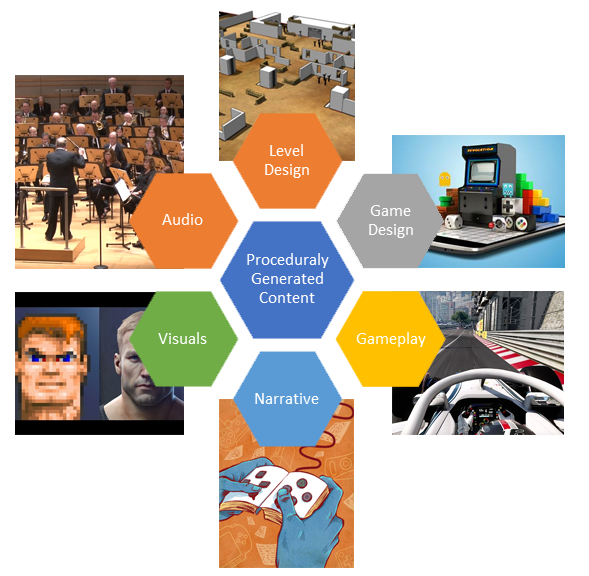
\includegraphics[width=0.6\textwidth]{img/pcg_areas.png}
    \caption{Areas de PCG en videojuegos}
    \label{figure:pcg_areas}
\end{figure}

\subsubsection{Diseño de niveles}
\label{subsection:LevelDesign}

La area del desarrollo de niveles es una de las populares en PCG debido a que
los niveles son la parte escencia de un juego debido a que es el area sobre el
cual un jugador puede interactuar, la representacion de estas areas se puede dar
desde imagenes en 2D simplemente con el alto y ancho de los objetos hasta
elementos en 3D que abarquen tambien el grosor de los objetos.

Debido a que los niveles son escencialmente el area principal de interaccion en
un videojuego estos deben de considerar los aspectos funcionalidad y estetica
para que exista una buena interaccion y sea llamativo a los usuarios, de esta
manera se pueden crear areas con tonos oscuros y ambiente tetrico para entregar
un nivel con tematica de terror, la generacion de niveles de juego es un tema
reciente en el ambito de investigacion debido a los elementos que se deben de
tener en cuenta sin embargo dentro del ambito de videojuegos, es un elemento
comunmente utilizado, algunos ejemplos recientes siendo Spelunky, Minecraft,
Disgaea.

Primero tenemos el juego de plataforma Spelunky desarrollado por Derek Yu, el
juego consta de multiples niveles alrededor de cinco diferentes areas, cada area
con un estilo diferente (niveles con hielo, lava, etc.) en este juego los niveles
que recorre el jugador son desarrollados de manera procedural por diferentes
algoritmos dependiendo el area en la que se encuentre el juegador.

El segundo ejemplo es un videojuego desarrollado por Markus Persson llamado
Minecraft, este juego consta de un area estilo caja de arena en donde el jugador
puede realizar las acciones que quiera, las estructuras estan definidas en
manera de bloques con diferentes texturas y propiedades que el jugador puede
utilizar para construir diferentes cosas, la manera en como se utiliza la
generacion de contenido es mediante la generacion de todo un nivel al iniciar el
juego de tal manera que se utiliza una semilla de generacion y se utiliza el
metodo \textit{Perlin Noise} 3D con interpolacion lineal para genrar los biomas,
elementos y entidades que conformaran el nivel.

Finalmente tenemos el juego Disgaea desarrollado por Nippon Ichi Software, este
es un juego de estrategia por turnos en donde el objetivo es eliminar a todos
los enemigos en un mapa para continuar al siguiente, la manera en como se
utiliza la generacion de contenido procedural es en una seccion extra del juego
en donde se puede entrar a un arma para completar niveles gradualmente mas
dificiles para darle mas poder a dicha arma, en esta parte los niveles que se
encuentra el jugador son generados proceduralmente tomando en cuenta las alturas
de las partes donde se puede caminar y la colocacion de los enemigos en el mapa
\ref{figure:DisgaeaIW}, para la generacion se toma en cuenta el nivel del arma y
su rareza, mientras mas altos sean estos valores de igual manera los nievels
generados seran mas dificiles.

\begin{figure}
    \centering
    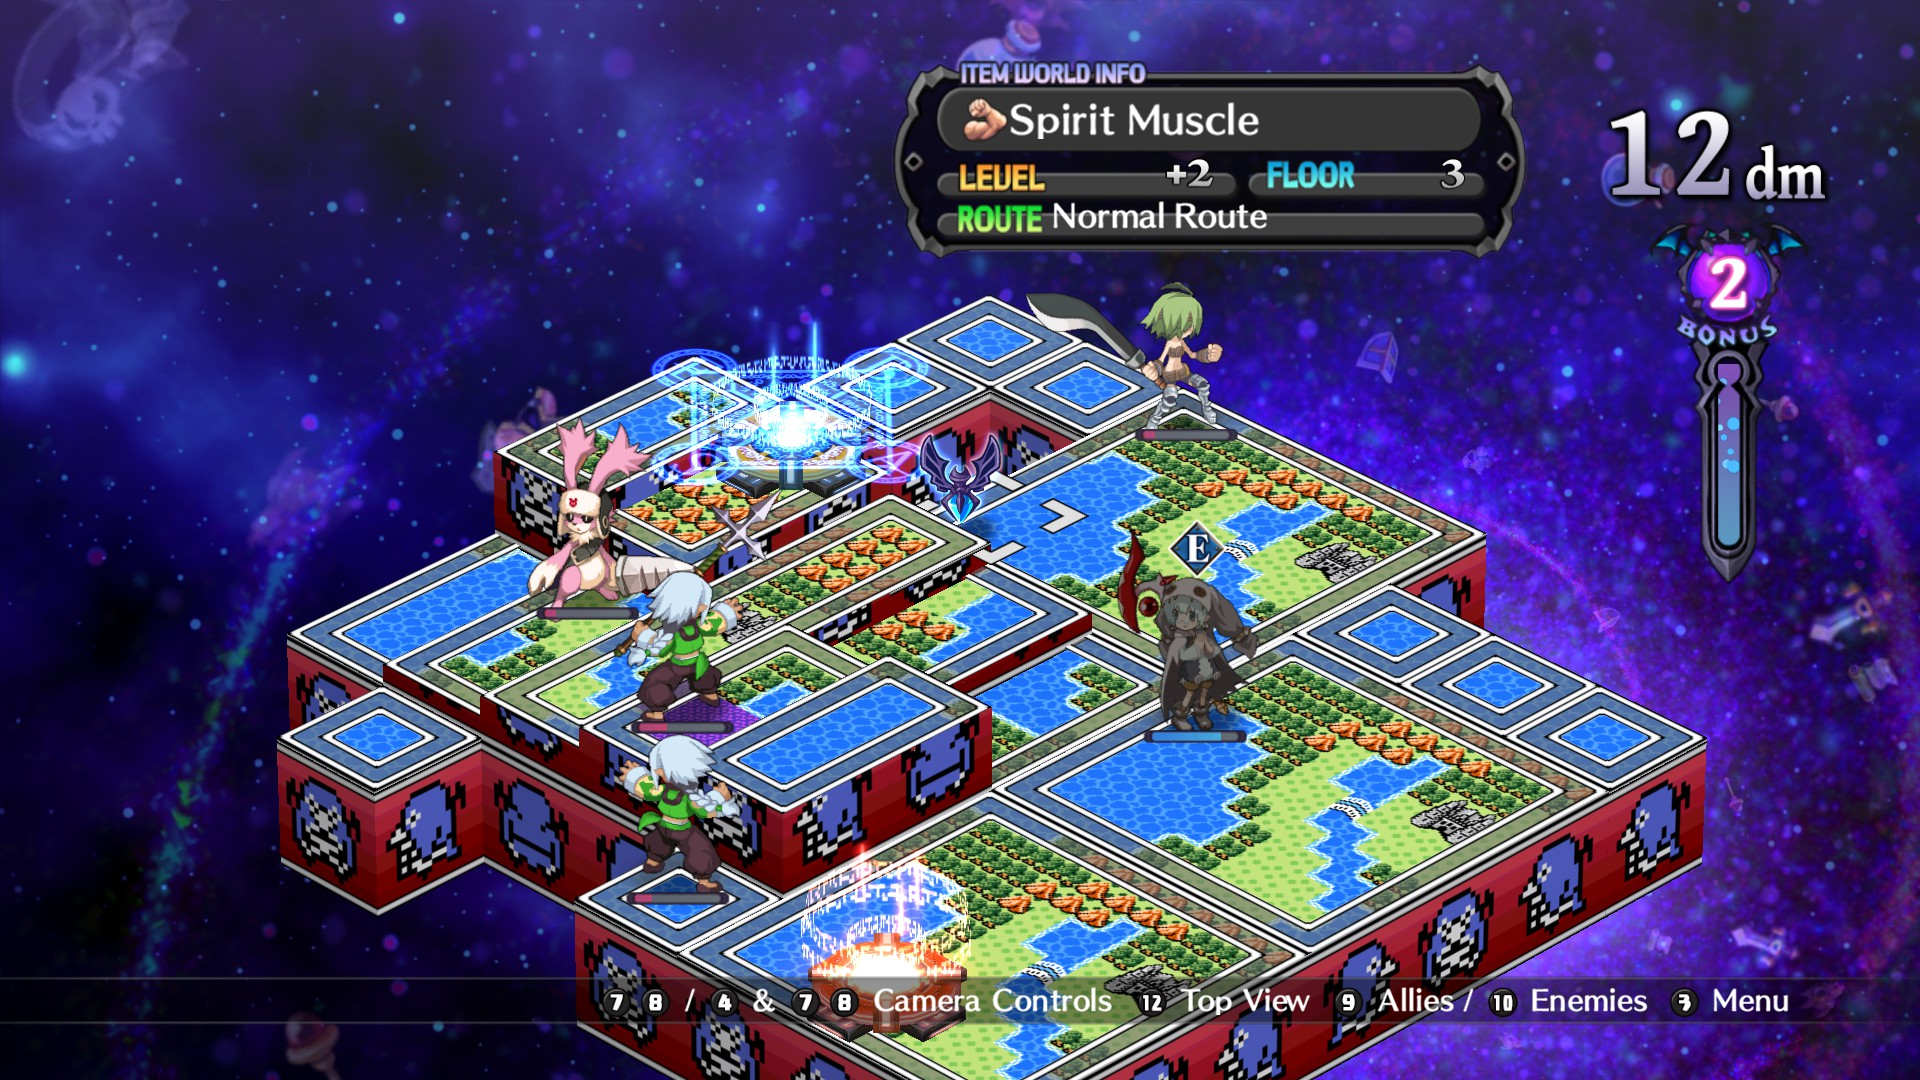
\includegraphics[width=1.0\textwidth]{img/DisgaeaIW.png}
    \caption{Nivel generado en el juego Disgaea}
    \label{figure:DisgaeaIW}
\end{figure}

\subsection{Gráficos}
\label{subsection:Visuals}

La area de desarrollo de graficos se encarga principalmente de generar las
representaciones visuales de los juegos debido a que la mayor parte de los
juegos llevan una parte visual a menos que no se requiera, es necesario generar
una imagen que denote lo que se quiere dar a entender en un juego, de esta
manera se le brinda al jugador un nivel mas de inmersion en la situacion
mediante el uso de paletas de colores o imagenes en pantalla que puedan
representar mejor las situaciones que se presentan.

El ambito de generacion de graficos ah sido uno de los mas explotados debido a
que es posible generar graficos desde simples representaciones de 8 bits como
representaciones photorealisticas de los eventos u objetos presentes en un
juego, tal es el caso explicado en el paper de Risi S. et al.\cite{Risi2012} en
donde utilizan una red de produccion de patrones composisionales (CPPN por sus
siglas en ingles) la cual es una variante de las redes neuronales artificiales
(ANN) regulares, utilizando esta red se busco modificar un circulo de tal manera
que la resultante de tal modificacion creara un patron en forma de una flor, de
igual manera la forma de crear diversidad en los tipos de flores generadas fue
mediante el uso de la neuroevolucion de topologias aumentativas (NEAT) mediante
el cual las redes generadas se alteraban mediante la modificacion de conecciones
entre neuronas y la adicion de nuevos nodos de tal manera que se buscaba un
nivel adecuado de complejidad para las redes que generaron diferentes tipos de
patrones de flores.

Mientras que un segundo paper escrito por Erin J. et al.\cite{Hastings2009} en
el cual presentan un nuevo algoritmo de generacion de contenido llamado
neuroevolucion de topologias aumentativas para generacion de contenido (cgNEAT)
el cual se encarga de generar contendio grafico y contenido del juego deacuerdo
a las preferencias de un jugador mientras el juego esta en ejecucion, para la
evaluacion del contenido generado se desarrollo un juego multijugador en linea
llamado \textit{Galactic Arms Race} en el cual la cgNEAT se encarga de generar
contenido para todos los jugadores y ellos eran quienes proveian la
retroalimentacion del funcionamiento del algoritmo.

\subsection{Audio}
\label{subsection:Audio}

El ambito de generacion de audio en videojuegos se puede considerar como un
punto opcional dependiendo del juego que se este desarrollando sin embargo el
audio juega un papel importante en la experiencia que se le brinda a un jugador
dentro del juego debido a que mediante el uso de componentes sonoros se pueden
influir las emociones que se quieren mostrar en lugares especificos, desde cosas
simples como el uso de sonidos de objetos como escuchar un teclado siendo
utilizado hasta la utilizacion de pistas de audio en areas o momentos clave del
juego para demostrar momentos dramaticos, tristes o de accion. 

Cabe mencionar que es posible utilizar instrumentos musicales o la
implementacion de orquestas para de igual manera generar estos ambientes sin
embargo algunos utilizan este tipo de generacion para crear pistas que sean
capaces de adaptarse a los sucesos que transcurren en el momento [Ref 220, 128
del "AI and Games"] de igual manera existen metodos para generar contenido
mediante el uso de pistas de audio, tal el caso de [Ref Audio Surf].

Finalmente tenemos \textit{Mezzo} desarrollado por Daniel B. este paper muestra
un programa de computadora del mismo nombre diseñado con el fin de generar
musica de la era romantica que puede ser utilizada en juegos de computadora, el
software fue desarrollado con el proposito de poder darle mas expresividad a
eventos que ocurren en juegos de computadora, esto es mediante el uso de los
elementos presentes en la escena como las partes que conforman la piexa musical,
para esto sus acciones son traducidas como diferentes cantidades de tension
armonica lo cual permite que la pieza musical corresponda al estado del juego
asi como a las acciones que realizan los personajes.

\subsection{Narrativa}
\label{subsection:Narrative}

El ambito de generacion de narrativa en videojuegos se encarga de manera basica
de generar historias que tengan sentido y sean entretenidas, el uso de PCG para
el ambito de narrativa se ah tomado de diferentes angulos, el primero es
sencillamente crear la historia del lugar en donde se desarrollan las cosas,
esto es generar toda la historia desde un punto especifico y asi crear una
"linea" de accion que un jugador debera seguir, mientras que otro de los
aspectos es la generacion de historia que se adapte a las acciones del jugador,
esto es, que a medida que el jugador progrese en un juego realizando acciones
especificas el juego adapte la historia a generar deacuerdo a dichas acciones.

Algunos ejemplos de este ambito de generacion se muestran en (Ref Facade), (Ref
Versu) y (Ref Blood y Laurels)

\subsection{Reglas y Mecanicas}
\label{subsection:rulesandmechanics}

Las reglas y mecanicas de un juego proveeen de un marco de trabajo en el cual el
jugador puede realizar acciones y el como debe de influenciarlas hacia un
objetivo final, las reglas y mecanicas de un juego pueden variar dependiendo del
tipo de juego que se trate, por ejemplo en juegos de estilo plataforma la regla
de terminacion puede ser simplemente llegar hasta cierto punto del nivel
mientras que las macanicas pueden incluir saltar, correr o agacaharse, este
conjunto de reglas permite que el jugador no realize acciones no preevistas por
los programadores y de tal forma limita a un jugador a cierca cantidad de
acciones y consecuentes posibles las cuales debera de aprovechar de diferentes
maneras para continuar.

Mientras que el uso de reglas permite tener un juego mas balanceado algunas
ocasiones el cambiar el conjunto de reglas permite crear diferentes tipos de
juegos, tomando el ejemplo anterior es posible que un juego de plataformas se le
permita a un jugador volar en un nivel lo cual provocaria que las mecanicas se
requieran acomdar a esta nueva habilidad y de igual manera los niveles de un
juego se tengan que reimaginar de tal modo que ahora se pueda utilizar en
ciertas o se coloquen lugares que solo se pueden acceder con esa habilidad por
ejemplo la transicion de reglas y mecanicas entre los juegos Super Mario Bros.
(Nintendo, 1985) y Super Mario World (Nintendo, 1990).

Para la evaluacion de la generacion de mecanicas y reglas de un juego existen
diferentes metodos a utilizar, el primero se basa en el balance de las reglas es
decir en caso de ser un juego para dos o mas jugadores el objetivo de evaluar
seria que todos los jugadores tengan las mismas probabilidades de ganar
utilizando las mecanicas del mismo juego, mientras que otra manera de evaluar
seria mediante la facilidad que tienen las mecanicas de ser aprendidas por los
jugadores.

En cuanto a ejemplos de este tipo de generacion se encuentran algunas
investigaciones academicas tales como la de Ludi (Ref Ludi num76) otro caso fue
escrito por Togelius et al. (Ref Togelius num716) mientras que un ultimo caso es
el de Nielsen et al. (Ref Nielsen num492).

\subsection{Juegos}
\label{subsection:games}

Mientras que las facetas de generacion anteriores se han enfocado en aspectos
especificos de juegos mientras que en este aspecto en particular se toma un
enfoque global, esto es desde la generacion de partes visuales hasta la 
generacion de bandas sonoras, esto demuestra como todos los aspectos de un
juegose relacionan unos con otros, un ejemplo de esta relacion seria tomar un
juego en particular y agregar acciones que originalmente no exitian, para poder
agregar estas acciones se debe de considerar el aspecto visual, es decir el como
debera de representarse visualmente tal accion, aspectos de sonidos en caso de
que una accion requiera de algun efecto de sonido que represente tal accion,
utilizando el ejemplo de agregar la mecanica de volar, el aspecto visual se
representaria en un cambio visible en el personaje controlado, por ejemplo,
dibujar alas y que se vea una animacion de movimiento al volar, en el caso del
aspecto del sonido el aleteo o movimiento generado por dichas alas al estar
volando puede tener un sonido unico para identificarlo.

Para este caso existen diferentes maneras de intentar generar juegos nuevos, tal
es el caso de Game-O-Matic (Ref Game-o-matic num723), otra investigacion realizada
por Nelson et al. (Ref Nelson num484), finalmente uno de los mejores generadores
de juegos lleva en nombre de ANGELINA (Ref ANGELINA num135-137).

Los anteriores generadores a pesar de no ser perfectos han permitido dar un gran
paso en la generacion de contenido o mas bien en la generacion de juegos, sin
embargo aun falta controlar aspectos que permitan que las generaciones de tal
contenido logren involucrar todos los aspectos de la generacion de contenido,
esto podria darse mediante el uso de multiples agentes que contantemente evaluen
los aspectos generados pero que al mismo tiempo logren comunicarse unos con
otros y poder evaluar los juegos generados de manera mas amplia.

\section{Algoritmos Geneticos}
\label{section:genetic-algorithms}

Los algoritmos geneticos (Genetic Algorithm, GA por sus siglas en ingles) son
algoritmos inspirados en la evolucion Darwiniana y utilizados para la
optimizacion de procesos, fue introducido por John Holland en 1975
\cite{Holland1975}, los GA son metodos de optimizacion y busqueda basados en los
principios de la seleccion natural y genetica, la manera de representarlos es
mediante un grupo de individuos que representan posibles soluciones a un
problema y mediante el uso de operadores geneticos estos individuos se cruzan y
evolucionan para acercarse mas al objetivo, el cual puede ser minimizar o
maximizar un valor resultaado de un sistema.

En otras palabras un GA es un metodo para resolver problemas de optmizacion

Deacuerdo a una explicacion proporcionada por Whitley en uno de sus articulos
\cite{Whitley1994}, un algoritmo genetico (GA) son algoritmos de optimizacion
inspirados en el proceso natural de evolucion. Por esta razon los GAs son
considerados como parate de una sub-area de algoritmos de optimizacion llamada
algoritmos evolutivos. La manera en como funciona un GA es que se propone tener
un conjunto inicial de posibles soluciones a problema, estas soluciones son
llamadas poblacion dentro del algoritmo. Cada una de estas soluciones propuestas
lleva el nombre de individuos y en ocaciones se definen como cromosomas. Esta
poblacion es evaluada mediante el uso de una funcion de aptitud encargada de
determinar el rendimiento de cada uno de los individuos como una de las posibles
soluciones para el problema que se esta tratando. Este tipo de problemas
comunmente involucran encontrar un conjunto de parametros que permitan minimizar
o maximizar los resultados obtenidos en un sistema.

El proceso que se realiza en un GA se describe de la siguiente manera, primero
la poblacion es sometida a un proceso de evolucion que involucra la realizacion
de cruces entre los individuos de la poblacion que tienen el mejor rendimiento
en la generacion, de igual manera aquellas soluciones que tengan un mal
desempeño deacuerdo a la funcion de aptitud son removidos de la lista de la
poblacion para las generaciones subsecuentes. El proceso de cruce de individuos
se realiza mediante la recombinacion de geners en los cromosomas de los
individuos seleccionados los cuales son seleccionados en base a sus resultados
en la funcion de aptitud siendo aquellos que llevaran a cabo los cruces los
mejores. Este proceso mencionado se repite durante un numero determinado de
iteraciones las cuales llevan el nombre de generaciones.

El objetivo de los GAs asi como en otros algoritmos evolutivos es que, mientras
las generaciones van pasando la poblacion comenzara a volverse mas apta y se
encaminara a cierto punto o valor que se espera sea el indicado para resolver un
problema, sin embargo, es comun que ninguno de los individuos logre llegar a una
solucion optima para el problema presentado. Sin embargo, al ejecutar el
algoritmo multiples veces el algoritmo evolutivo lograra proveer varios
resultados diferentes, esto es debido a que la poblacion inicial en cada ciclo o
ejecucion se genera de manera aleatoria. Por esta razon, los algoritmos
evolutivos y por ende los algoritmos geneticos son considerados como algoritmos
de busquedas meta-heuristicas, debido a que son capaces de encontrar soluciones
casi optimas para problemas en donde los algoritmos evolutivos no sean
involucrados de manera directa, ademas de esto los algoritmos evolutivos tambien
son considerados algoritmos estocasticos debido a la aleatoriedad que conlleva
utilizar este tipo de algoritmos \cite{Harik1999}.

\section{Multi-agent Systems and Models}
\label{section:multi-agent-systems-and-models}

A multi-agent system is software that solves a problem using agents. Agents can
be seen themselves as programs that interact with their environment, which may
include other agents. Agents in the proposed method in this paper follow the
structure suggested by Shoham in \cite{Shoham1993}, where agents have beliefs
and rules. Beliefs are used by agents to arrive to an interpretation of their
environment, and rules are used to arrive to actions to be performed by the
agent towards their environment. The agents in the system are constantly sensing
their environment to determine what actions to take according to their beliefs
and rules. Multi-agent systems have the objective of solving a practical
problem, unlike agent-based models which are more focused to providing a
simulation of a problem.

As mentioned before, agents can also be used to create agent-based models. These
models are used to represent a problem so a human being can analyze it and infer
new knowledge from it, or it can be used to better understand a problem.

The proposed method in this paper is both a multi-agent system and an
agent-based model. It is a multi-agent system in the sense that it can be used
to create a trading strategy, and it is an agent-based model because the agents
in the system can be analyzed to understand the state of the market that is
serving as the system's environment.
